\documentclass[border=5pt,tikz]{standalone}
\tikzset{
  ctrlpoint/.style={%
    draw=gray,
    circle,
    inner sep=0,
    minimum width=1ex,
  }
}
\newcommand\Bezier[4]{% \bezier (lowercase 'b') was already defined elsewhere
  \node (p1) [ctrlpoint,label=90:$P_1$] at (#1) {};
  \node (p2) [ctrlpoint,label=90:$P_2$] at (#2) {};
  \node (p3) [ctrlpoint,label=90:$P_3$] at (#3) {};
  \node (p4) [ctrlpoint,label=90:$P_4$] at (#4) {};
  \draw [gray] (p1) -- (p2) -- (p3) -- (p4);
  \draw [blue] (#1) .. controls (#2) and (#3) .. (#4);
}
\begin{document}
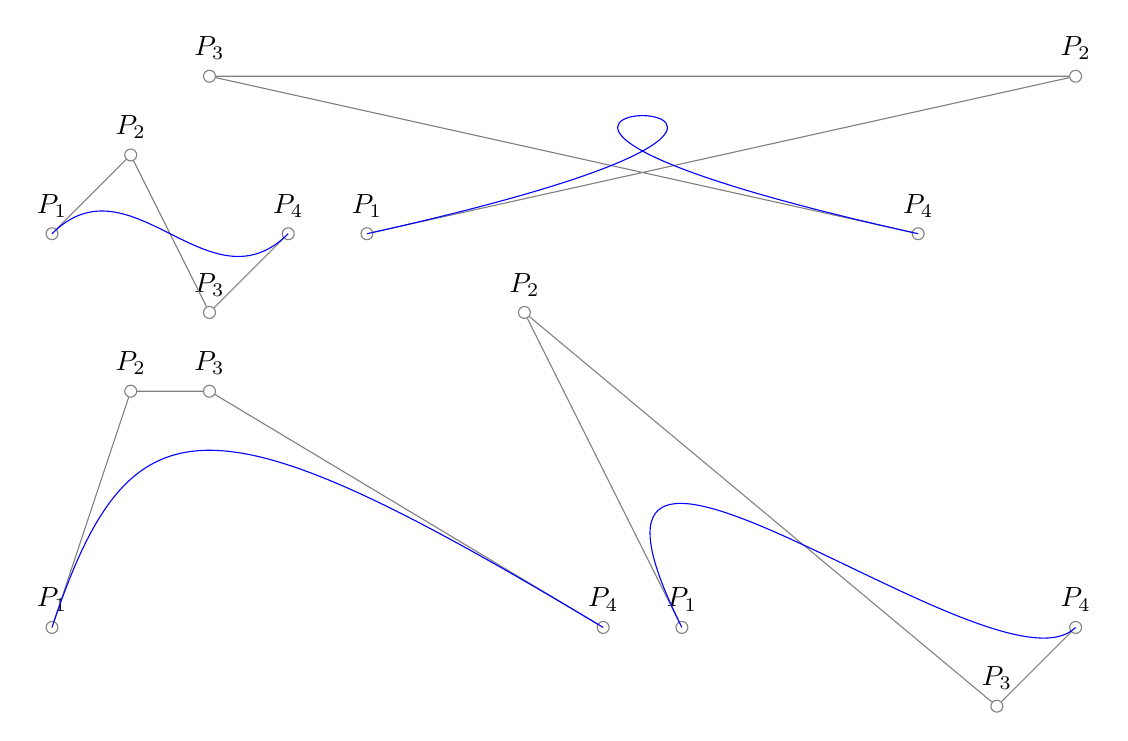
\begin{tikzpicture}
  \Bezier{0,0}{1,1}{2,-1}{3,0}
  \begin{scope}[xshift=4cm]
    \Bezier{0,0}{9,2}{-2,2}{7,0}
  \end{scope}
  \begin{scope}[yshift=-5cm]
    \Bezier{0,0}{1,3}{2,3}{7,0}
  \end{scope}
  \begin{scope}[xshift=8cm,yshift=-5cm]
    \Bezier{0,0}{-2,4}{4,-1}{5,0}
  \end{scope}
\end{tikzpicture}
\end{document}